\section{Materials and methods}

\subsection{Participants}

Eight naive participants (three male, five female), aged between 22 and 29 years, provided written informed consent to participate in the experiment. All participants were free of any known vestibular or neurological disorder and had normal or corrected-to-normal visual acuity. Participants never received any feedback about their performance.

\subsection{Experimental setup}

A motorized linear sled (see \cite{clemens2012} for details) was used to laterally translate participants following a minimum jerk profile of fixed duration (1 \si{\second}) and amplitudes ranging from 1 to 27 \si{\centi\metre}. Participants were seated on the sled such that the inter-aural axis aligned with the motion axis. They were restrained using a five-point seat belt and a chin rest. In addition, the head was held in place using an ear-fixed mold. Auditory cues were suppressed using white noise presented through in-ear headphones. Experiments were conducted in complete darkness except for visual fixation points, projected by a laser pointer on a black bar 50cm in front of the participant at eye level. Laser pointers used to project body-fixed targets were attached to the sled. Those used to project world-fixed targets were mounted on the wall behind the sled.

Eye movements were recorded at 500 \si{\hertz} using an EyeLink II (SR Research, Kanata, Canada) system whose cameras were mounted to the sled and therefore remained stable with respect to the head during the entire experiment. Because the head and body positions were fixed during the experiment, the orientation of the eyes within the head, as measured by the tracker, was equivalent to the orientation of the eyes in space. The eye tracking system was calibrated before each session using 11 evenly spaced calibration points ranging from -22 to \siang{22}. We used linear regression to link EyeLink measurements to gaze angles.

\subsection{Paradigm}
We used a two-alternative forced choice (2-AFC) task to measure perceived linear self-motion across three different eye fixation types: world-fixed, body-fixed, and unconstrained (free) fixation. We refer to these as world, body and free, respectively. A trial contained two sequential translation intervals of equal duration (1 \si{\second}) and in the same direction (either leftward or rightward). Different fixation types were presented in the two translation intervals. Participants were instructed to judge whether the translation during the second interval was longer or shorter compared to the first interval. They were additionally instructed to always look at the fixation point when it was visible; no instructions were given for when the fixation point was switched off (i.e. during free fixation).

\begin{figure}
    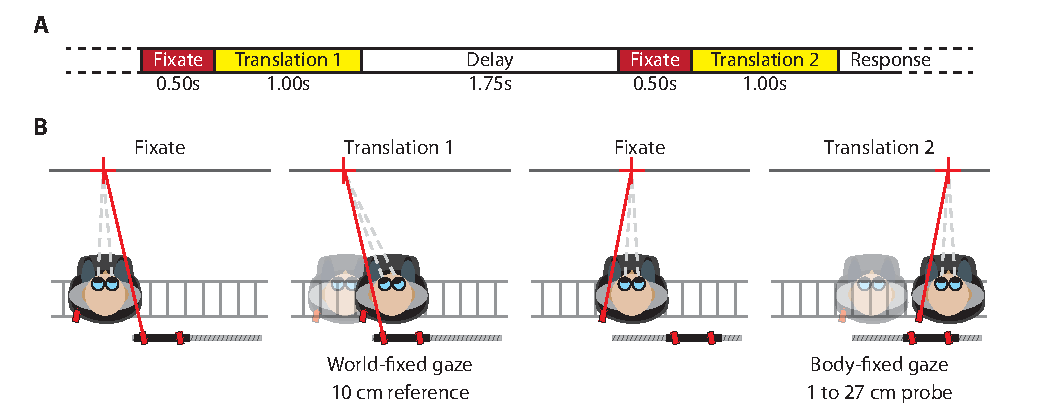
\includegraphics[width=1.0\textwidth]{src/paper3/figure1.pdf}

    \caption{\panelref{A} Time course of key events within a single trial. In each of the two intervals, a 0.50 \si{\second} fixation period (red) precedes the lateral translation (yellow). A 1.75 \si{\second} long delay period (shown in white) separates the two intervals. After the second translation, the participant responded whether this second translation was longer or shorter than the first. \panelref{B} Top-view illustrating key events during a body vs. world trial. First panel: participant fixates the world-fixed target (red cross) at the start of the first interval. Second panel: translation with world-fixed fixation target. Third panel: body-fixed fixation at start of second fixation interval. Fourth panel: translation with body-fixed fixation in second interval.}
    \label{p3:fig1}    
\end{figure}

The time evolution of a single trial is shown in \figref{p3:fig1}. Each trial started with the onset of a central fixation point (i.e. aligned between the eyes) for 0.5 \si{\second}. Subsequently, the first translation interval commenced.  Depending on the fixation type, the fixation point remained visible (world and body) or was extinguished (free) during the translation interval. The trial shown in the figure depicts the reference translation of 10 \si{\centi\metre} with world fixation. After this first interval, a delay followed in which the participant was kept in complete darkness for 1.75 \si{\second}. Then, the central fixation point reappeared, followed 0.5 \si{\second} later by the second interval, in which the probe translation was presented with amplitudes in the range of 1 to 27 \si{\centi\metre}. The fixation type in the probe interval was always different than in the associated reference interval (the trial in \figref{p3:fig1} illustrates body fixation). After the second interval, the participant had to indicate using a joystick whether he or she perceived the second translation as longer or shorter than the first.

\begin{table}
    \begin{tabular}{llll}
    Comparison & Reference & 1st interval & Direction \\
    \hline
    Body vs. world & Body & Reference & Right \\
    & & & Left \\    
    & & Probe & Right \\
    & & & Left \\
    \cline{2-4}
	& Body & Reference & Right \\
    & & & Left \\    
    & & Probe & Right \\
    & & & Left \\
    \hline
    Body vs. free & Body & Reference & Right \\
    & & & Left \\    
    & & Probe & Right \\
    & & & Left \\
    \cline{2-4}
	& Free & Reference & Right \\
    & & & Left \\    
    & & Probe & Right \\
    & & & Left \\
    \hline
    World vs. free & World & Reference & Right \\
    & & & Left \\    
    & & Probe & Right \\
    & & & Left \\
    \cline{2-4}
	& Free & Reference & Right \\
    & & & Left \\    
    & & Probe & Right \\
    & & & Left \\    
    \end{tabular}

    \caption{List of the three main comparisons that we tested. The (10 \si{\centi\metre}) reference movement was presented in either the first or second movement interval. We also manipulated movement direction (leftwards or rightwards), yielding a total of 24 trial types.}

    \label{p3:tab1}
\end{table}

Thus, a trial consists of two translations with different fixation types; in the three main conditions we compare the body versus world, world versus free, and body versus free fixation types. For each main condition, we varied which fixation type served as the reference stimulus and the order in which reference and probe were presented, which gives a total of four variations per main condition (see \tabref{p3:tab1}). In addition we varied translation direction (either leftward or rightward on consecutive trials). The amplitude of the probe translation was adaptively chosen based on the participants' earlier responses \cite{kontsevich1999} to determine the point of subjective equality. This was done separately for all 24 trial types (3 main conditions x 2 reference stimuli x 2 reference/probe orders x 2 translation directions; see \tabref{p3:tab1}). A total of 25 trials were collected per trial type yielding a total of 200 trials for each of the three main conditions.

Trials were presented in three one-hour sessions. To prevent dark adaptation, we turned on the lights for 5 \si{\second} after every block of 6 trials, and for at least 30 seconds every 4 blocks. We made sure that each of the 24 unique trial types were presented once every 4 blocks. After each block, the adaptive procedure determined which translation amplitudes to test in the following block. To increase the number of data-points available to the adaptive psychometric procedure at the beginning of the experiment, we collapsed across translation direction and reference order for the first 10 trials. After those blocks the procedure ran separately for each of the 24 distinct trial types.

\subsection{Data analysis}

For each combination of the three main conditions, and the two reference/probe orders (see \tabref{p3:tab1}), we quantified the perceived probe translation by calculating the probability of the probe translation judged longer compared to the reference translation as a function of actual probe translation. We used a maximum likelihood fit of a cumulative Gaussian function to summarize the psychometric data:

\begin{equation}
\label{p3:eq1}
P(x) = \lambda + (1 - 2\lambda) \frac{1}{\sigma \sqrt{2\pi}} \int_{-\infty}^{x}{e^{-(y-\mu)^2 / 2\sigma^2}}dy,
\end{equation}

in which $|x|$ represents the size of the probe displacement. The mean of the Gaussian represents the point of subjective equality (PSE). The slope of the curve reflects the precision ($1/\sigma$) of reference-probe discrimination performance. Parameter $\lambda$, representing the lapse rate, accounts for stimulus-independent errors caused by subject lapses or mistakes and was restricted to small values ($\lambda < 0.06$). Fits were performed using the Psignifit toolbox \cite{wichmann2001,wichmann2001b}.

In order to elucidate the effects of eye movements on self-motion perception, we quantified eye movement during each sled movement. To this end, we first corrected eye movements for drift based on the initial fixations at the start of each trial when the sled was still stationary. Subsequently, these actual eye movements were normalized as a ratio ($g_i$) of the theoretical eye movements that would have occurred had the subject kept fixating the initial, world stationary, target location. Trials in which the normalized final eye position was more than two standard deviations away from the average normalized final eye position were excluded from further analysis. This was done separately for each subject and fixation type. Trials containing blinks were also removed. In total 12.6\% of all trials were rejected.

Using a simple cue integration model, we investigated whether inter-subject and inter-condition differences in the observed PSEs in conditions containing a translation under free fixation depend on actual eye movement behavior. For these analyses we used the normalized eye movements. Ideally, the normalized eye movement would be $g_i \approx 0$ for body fixation and $g_i \approx 1$ for world fixation. With free fixation, eye movements are expected to be in-between body and world, $0 < g_i < 1$, but the exact value is participant dependent. Variable $i$ represents either the reference ($r$) or probe ($p$) interval. We model perceived distance, $p_i$, as a weighted linear combination of a vestibular and an oculomotor estimate of translation (Eq. 2). We assume that the vestibular estimate is equal to the actual translation, $m_i$, and that the oculomotor estimate is equal to the actual translation scaled by the normalized eye movement, $g_i m_i$. We further assume that the weights sum to one, such that the weighting parameter $\alpha$ regulates the eye movement contribution and $1 - \alpha$ the vestibular contribution:

\begin{equation}
\label{p3:eq2}
p_i = g_i m_i \alpha + m_i (1 - \alpha)
\end{equation}

By definition, at the PSE the estimated translation of the probe displacement ($p_p$) is equal to the estimated translation of the reference displacement ($p_r$). By substituting both sides by the right hand side of \eqnref{p3:eq2} and using subscripts for reference ($r$) and probe translations ($p$), we obtain:

\begin{equation}
\label{p3:eq3}
g_r m_r \alpha + m_r (1 - \alpha) = g_p m_p \alpha + m_p (1 - \alpha)
\end{equation}

In this equation $m_r$ equals the actual reference translation of 10 cm and $m_p$ equals the measured PSE. After rewriting \eqnref{p3:eq3} into \eqnref{p3:eq4}, we performed linear regression to find the weight ($\alpha$) that minimizes the sum of squared errors ($\sum{\epsilon^2}$) over the body versus world and world versus body conditions only:

\begin{equation}
\label{p3:eq4}
m_p - m_r = \alpha ( g_r m_r - g_p m_r + m_p - m_r ) + \epsilon
\end{equation}

Next we used this subject specific $\alpha$ to predict the PSEs for the conditions containing a free-fixation. To this end we solved \eqnref{p3:eq3} for $m_p$ (\eqnref{p3:eq5}), which is an estimate ($\hat{m}_p$) of the PSE, and plugged in numerical values for the reference translation and the average normalized eye movements over the reference and probe trials.
                                                                                            \begin{equation}
\label{p3:eq5}
\hat{m}_p = \frac
	{g_r m_r \alpha + m_r (1 - \alpha)}
	{g_p \alpha + (1 - \alpha)}
\end{equation}

